\section{Scopo del documento}
Questo documento ha lo scopo di descrivere i requisiti del progetto "Sistema di monitoraggio ambientale" mediante dei diagrammi in Unified Modeling Language(UML) e tabelle strutturate. I requisiti espressi nel precedente documento utilizzando solo il linguaggio naturale, sono spiegati ulteriormente, supportati da dei linguaggi più formali e precisi: UML per quanto concerne i requisiti funzionali e delle tabelle strutturate per la descrizione dei requisiti non funzionali ed i vincoli imposti dal cliente.

\section{Requisiti funzionali}
Nella seguente sezione vengono riportati i requisti funzionali (RF) del sistema nel linguaggio UML, in particolare utilizzando vari tipi di Use Case Diagram (UCD).

\phantomsection
\subsection*{RF 2.1 Interazione con l'app}
\addcontentsline{toc}{subsection}{2.1 Interazione con l'app}

Nel menù c’è una voce dedicata alla selezione dell’area di interesse; una volta selezionata le
funzionalità dell’app riguarderanno ovviamente la zona scelta. Tali funzionalità sono:
\begin{itemize}
    \item Guida turistica sulla biodiversità (flora/fauna)
    \item Statistiche sulla valutazione rischi (RF. 3)
    \item Notifiche associate ai rischi (RF. 3 e 4)
    \item Storico popolazione/tempo di flora e fauna (RF. 5)
    \item Impostazioni generali: supporto multilingua, disattivazione notifiche, assistenza, informazioni sull’app e normative sui dati.
\end{itemize}

\phantomsection
\subsection*{RF 2.2 Sistema e Utenti}
\addcontentsline{toc}{subsection}{2.2 Sistema e Utenti}


\subsubsection*{\underline{\large{Utente generale}}}

\begin{figure}[ht]
    \centering
    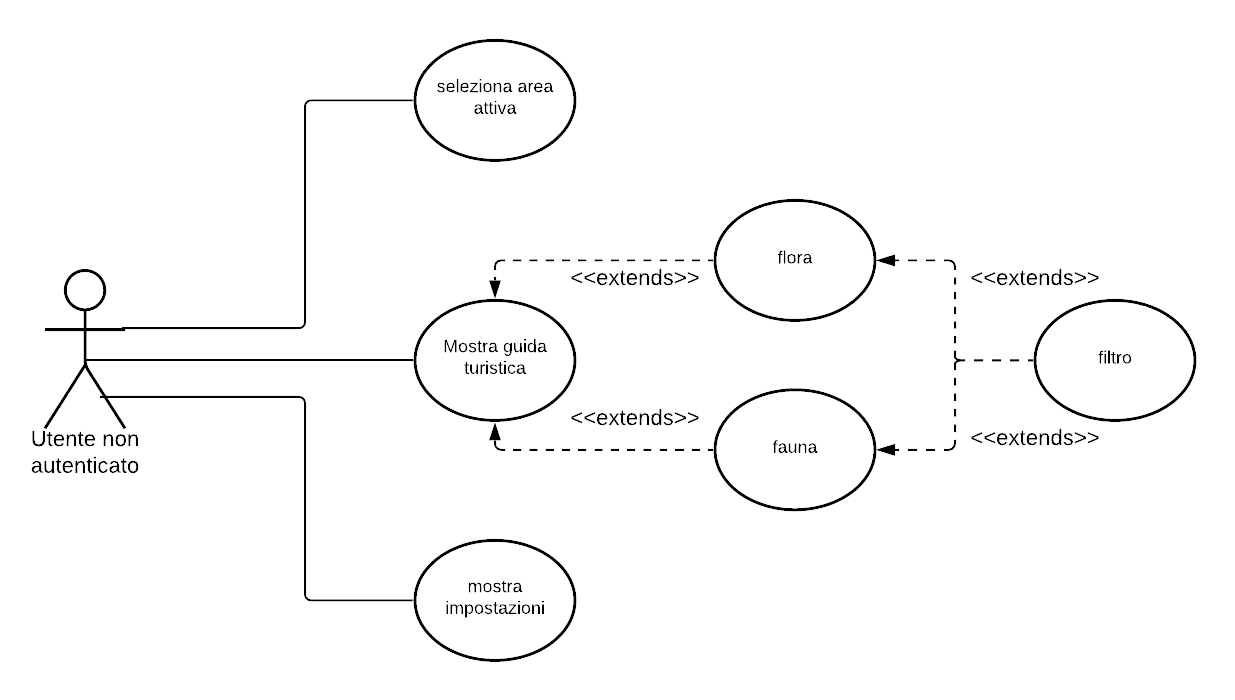
\includegraphics[scale=0.35]{Img/Utente_non_autenticato.png}
\end{figure}

\subsubsection*{Descrizione Use Case "seleziona area attiva"}
Questo use case descrive come l'utente può selezionare l'area in cui si trova.
\begin{enumerate}
    \item L'utente seleziona dal menù la voce "area attiva";
    \item Il sistema mostra la lista delle aree presenti nell'applicazione;
    \item L'utente seleziona l'area in cui si trova;
    \item Ora il sistema mostrerà le informazioni dell'area selezionata.
\end{enumerate}

\subsubsection*{Descrizione Use Case "mostra guida turistica"}
Questo use case descrive come vengono mostrate le informazioni di flora e fauna.
\begin{enumerate}
    \item L'utente seleziona dal menù la voce "flora" o "fauna";
    \item L'utente può applicare dei filtri: ordinamento (alfabetico, casuale), specie (protetta e non protetta) e popolazione (numero di esemplari: crescente o decrescente);
    \item Il sistema mostra tutte le specie presenti nell'ambiente;
    \item L'utente può selezionare una particolare specie per visualizzare una descrizione turistica.
\end{enumerate}

\subsubsection*{Descrizione Use Case "mostra impostazioni"}
Questo use case descrive cosa viene mostrato nelle impostazioni.
\begin{enumerate}
    \item L'utente seleziona dal menù la voce "impostazioni";
    \item Il sistema mostra una schermata dove l'utente può selezionare:
    \begin{itemize}
        \item disattiva notifiche;
        \item cambia lingua;
        \item assistenza;
        \item normative dati;
        \item informazioni app.
    \end{itemize}
\end{enumerate}

\subsubsection*{\underline{\large{Amministratore}}}

\begin{figure}[ht]
    \centering
    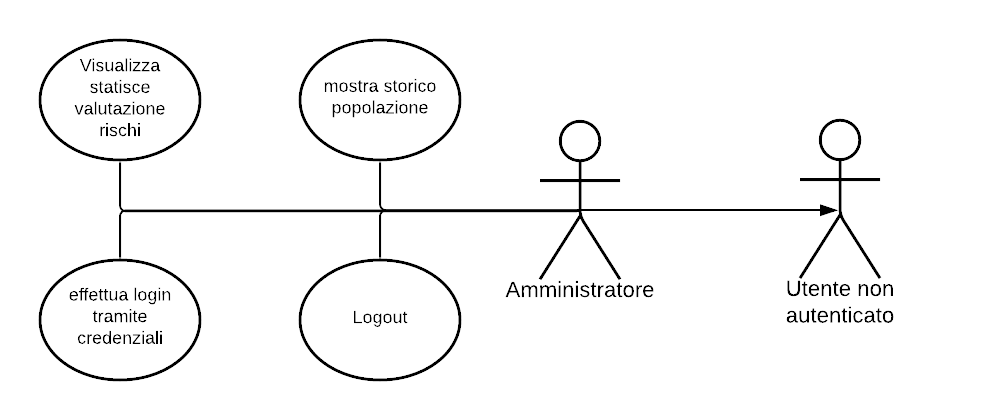
\includegraphics[scale=0.4]{Img/Amministratore.png}
\end{figure}

\subsubsection*{Descrizione Use Case "effettua login tramite credenziali"}
Questo use case descrive come avviene il login di un amministratore.
\begin{enumerate}
    \item L'amministratore fornisce agli sviluppatori un email valida;
    \item Gli sviluppatori creano un account per l'amministratore;
    \item L'amministratore dovrà effettuare il primo login utilizzando nome utente e OTP forniti via email;
    \item L'amministratore  seleziona dal menù la voce "login";
    \item L'amministratore deve inserire nome utente e password;
    \item Al primo login dovrà cambiare la password e successivamente ogni 30 giorni;
\end{enumerate}

\subsubsection*{Descrizione Use Case "visualizza statistiche valutazione rischi"}
Questo use case descrive come vengono mostrate le percentuali di rischio.
\begin{enumerate}
    \item L'amministratore seleziona dal menù "monitoraggio";
    \item Il sistema mostra a schermo le percentuali attuali dei vari rischi.
\end{enumerate}

\subsubsection*{Descrizione Use Case "mostra storico popolazione" \textbf{RF 2.5}}
Questo use case descrive come viene visualizzato lo storico della popolazione.
\begin{enumerate}
    \item L'amministratore seleziona dal menù "fauna";
    \item L'amministratore può applicare dei filtri: ordinamento (alfabetico, casuale), specie (protetta e non protetta) e popolazione (numero di esemplari: crescente o decrescente);
    \item Il sistema mostra tutte le specie presenti nell'ambiente;
    \item L'amministratore può selezionare una particolare specie per visualizzare le seguenti informazioni:
    \begin{itemize}
        \item istogramma popolazione/tempo (con scala del tempo selezionabile: anno, mese, giorno);
        \item mappa in cui è possibile visualizzare la posizione in tempo reale degli elementi specie selezionata presenti nell'area (se disponibile).
    \end{itemize}
\end{enumerate}

\subsubsection*{Descrizione Use Case "logout"}
Questo use case descrive come l'amministratore può effettuare il logout.
\begin{enumerate}
    \item L'amministratore ha a disposizione un pulsante nel menu chiamato "logout";
    \item L'amministratore può selezionare dal menù "area attiva";
    \item Se il sistema non identifica l'utente come amministratore nell'area selezionata viene effettuato il logout automatico.
\end{enumerate}

\phantomsection
\subsection*{RF 2.3 Monitoraggio e RF 2.4 Comunicazione}
\addcontentsline{toc}{subsection}{2.3 Monitoraggio e Comunicazione}
In questa sezione vengono descritte le azioni svolte dai seguenti attori:
\begin{itemize}
    \item Il sistema di calcolo probabilistico elabora i dati ricevuti dai sensori ambientali, come verrà spiegato successivamente;
    \item Il database memorizza i dati relativi alla flora, fauna, amministratori e i dati elaborati dal sistema di calcolo probabilistico;
    \item Il sistema di invio mail e di notifica si divide nei due casi espressi nelle pagine seguenti: disastri ambientali, fuga animali pericolosi.
\end{itemize}

\begin{figure}[ht]
    \centering
    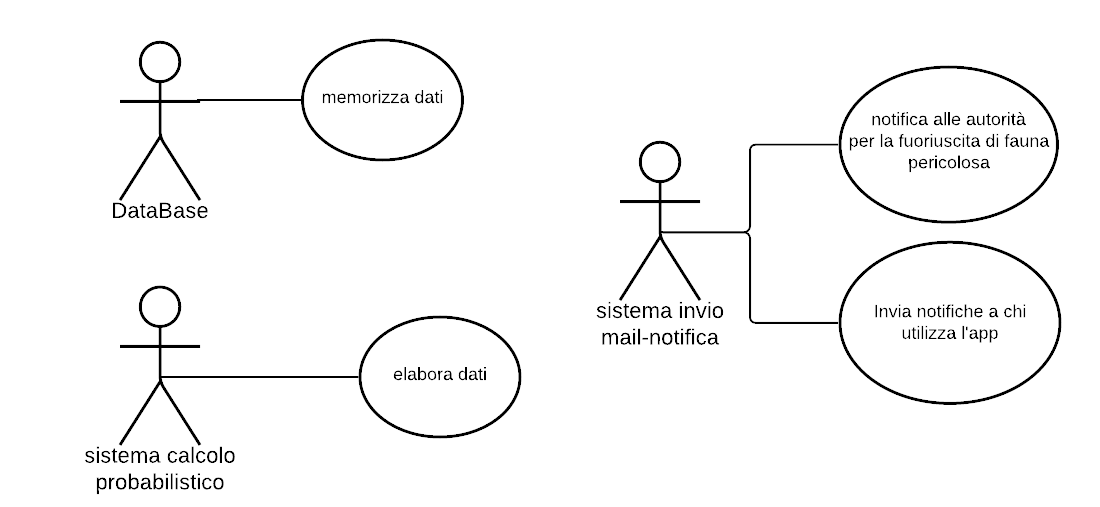
\includegraphics[scale=0.35]{Img/use_case_2_3_4.png}
\end{figure}

\pagebreak
\subsubsection*{Descrizione degli Use Case}

Il sistema di monitoraggio ambientale riceve dei dati elaborati sottoforma di percentuale dal sistema di calcolo probabilistico, elaborando i dati sulla probabilità dell'avverarsi dei seguenti rischi:
\begin{itemize}
    \item Allagamento
    \item Siccità
    \item Incendio 
    \item Svuotamento di risorse idriche
    \item Allarmi meteo
\end{itemize}
Nello schema sottostante viene descritta la \textbf{gestione dei rischi} da parte del sistema mediante Activity Diagram:

\begin{figure}[ht]
    \centering
    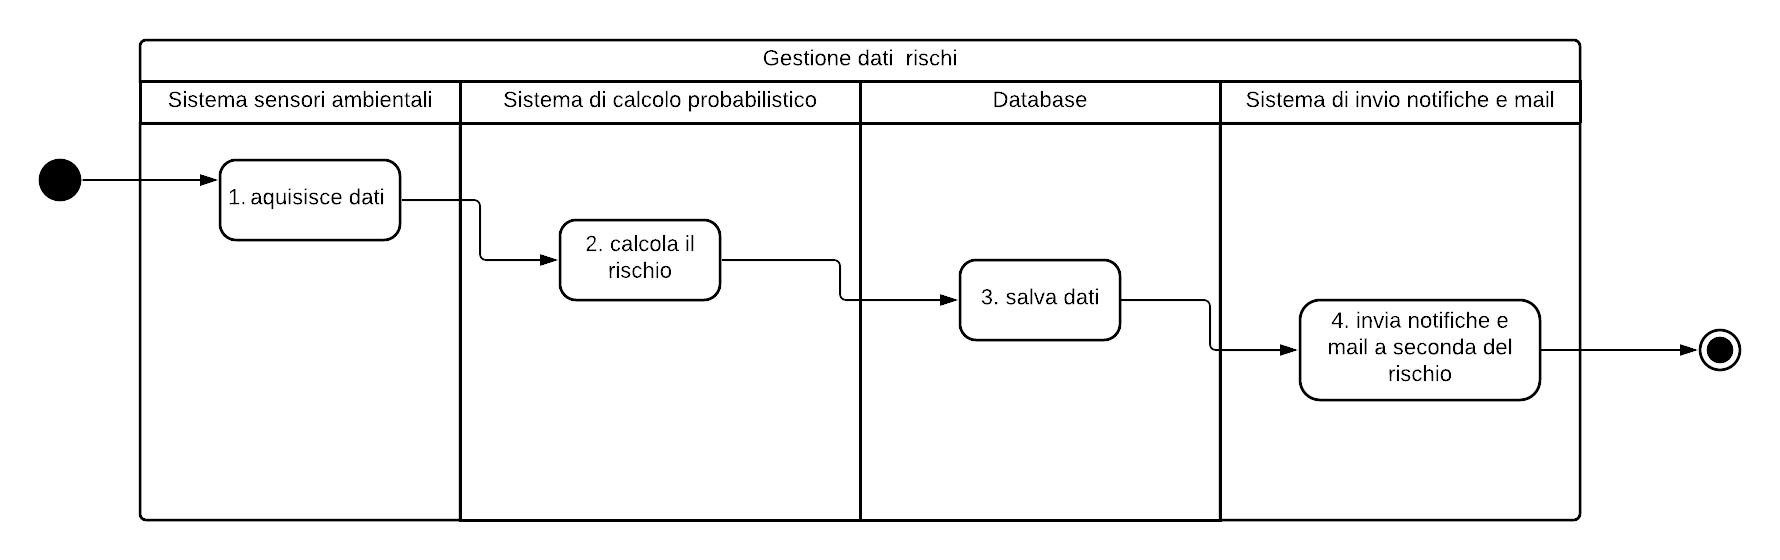
\includegraphics[scale=0.25]{Img/swim_gestione_rischi.png}
\end{figure}

La figura seguente, invece, descrive i vari casi a seconda delle analisi sul rischio ricevute. A ciascun livello sono associate determinate azioni.

\begin{figure}[ht]
    \centering
    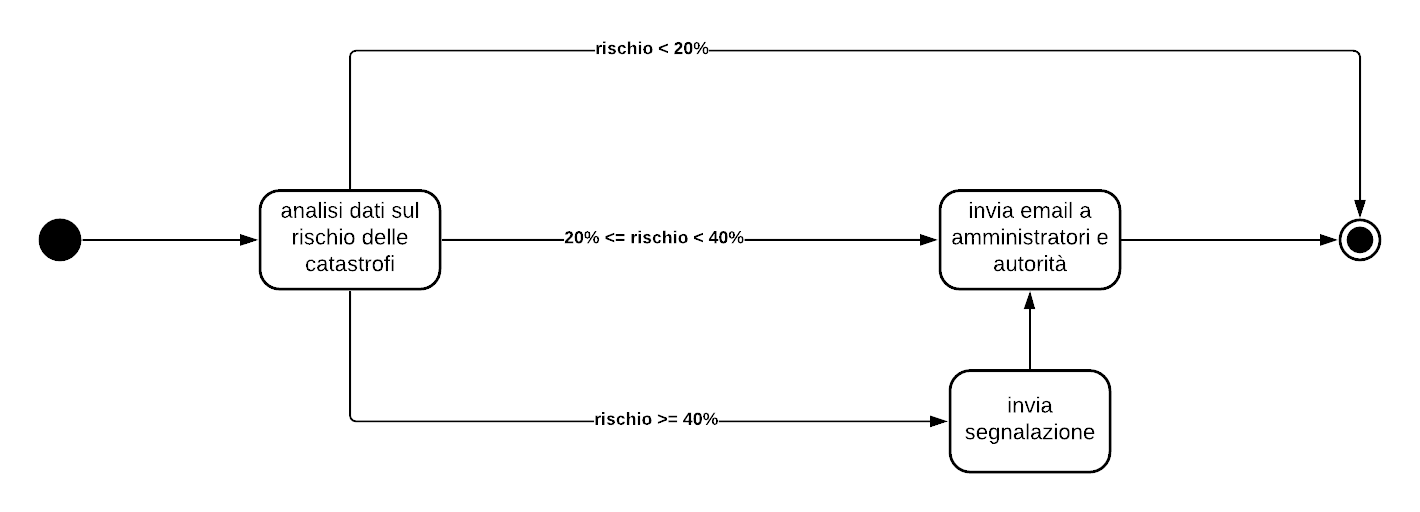
\includegraphics[scale=0.3]{Img/activity_rischi.png}
\end{figure}

\pagebreak

Il \textbf{sistema di sensori ambientali}, come precedentemente accennato, acquisisce dati e li fornisce al sistema di calcolo probabilistico. Il \textbf{sistema gps}, invece, indica la posizione e il numero di animali di medie e grandi dimensioni presenti nell'area, come spiegato nel diagramma seguente.

\begin{figure}[ht]
    \centering
    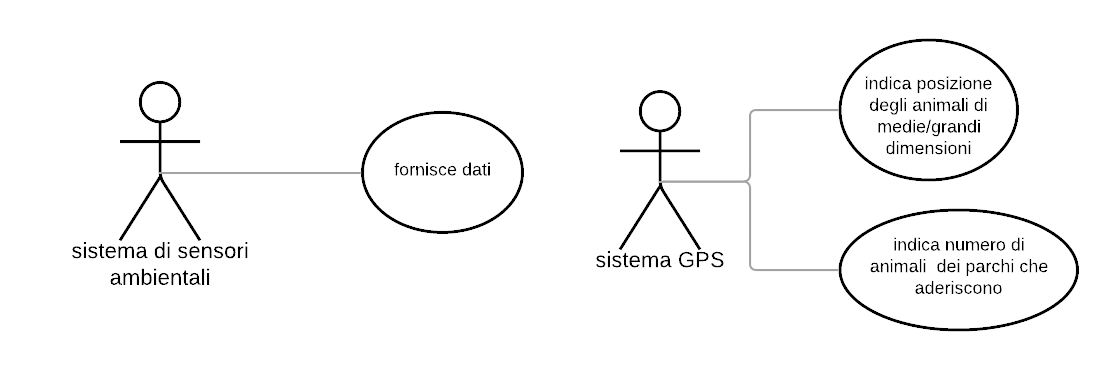
\includegraphics[scale=0.4]{Img/gestione_animali.png}
\end{figure}

\begin{figure}[ht]
    \centering
    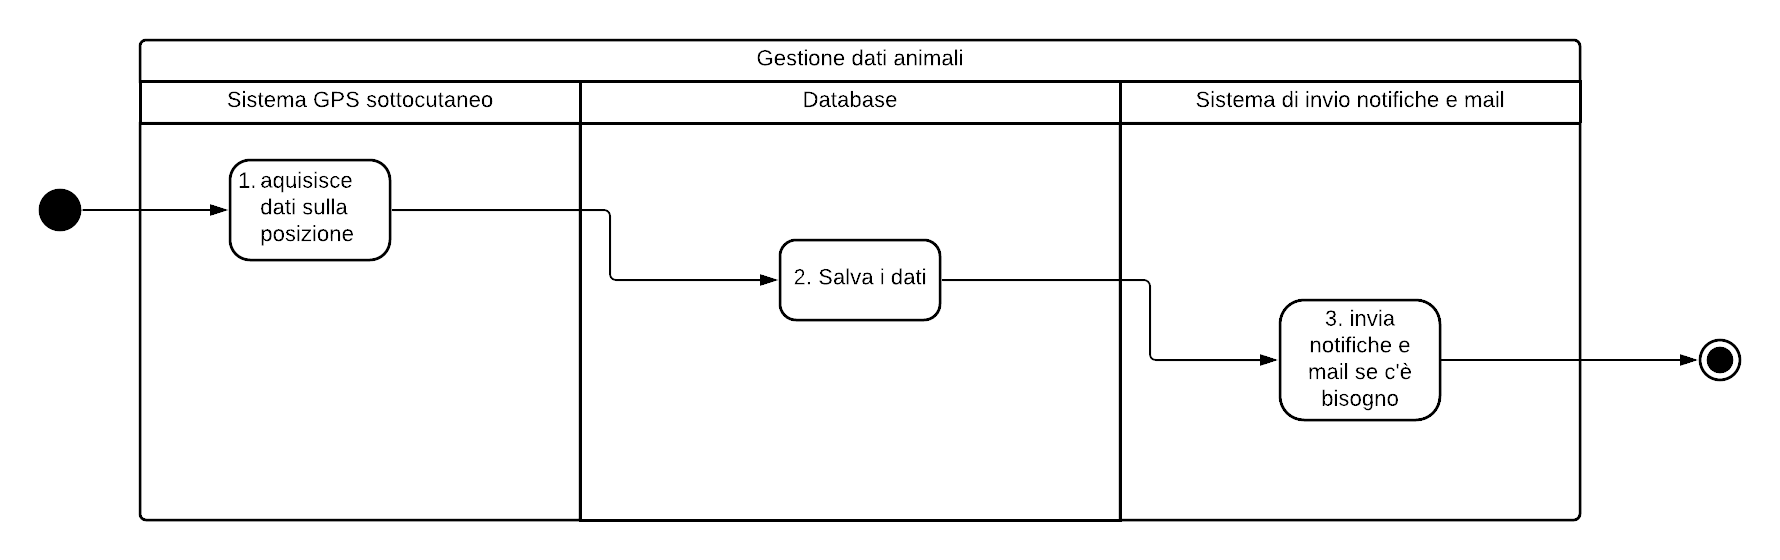
\includegraphics[scale=0.25]{Img/swim_gestione_animali.png}
\end{figure}

Il diagramma successivo analizza il caso in cui un animale fuoriesca dalla zona prestabilita.

\begin{figure}[ht]
    \centering
    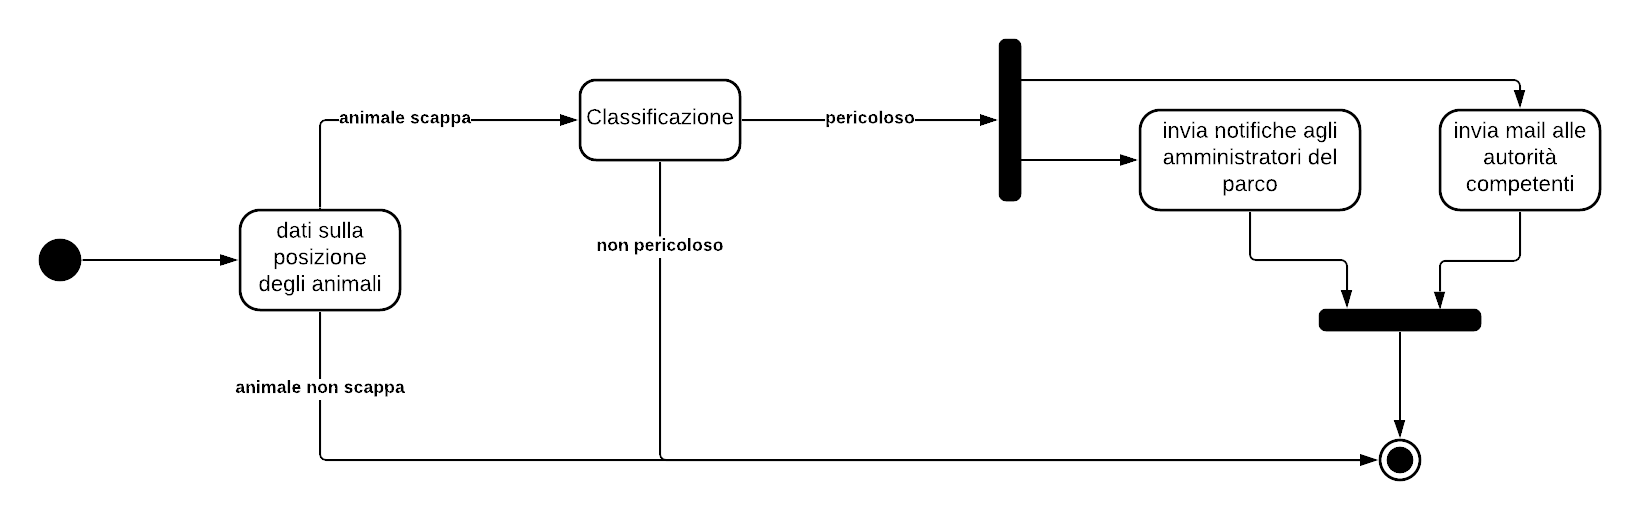
\includegraphics[scale=0.29]{Img/activity_animali.png}
\end{figure}